\documentclass[letterpaper,12pt,twoside]{book}
\usepackage{lecture-notes}

% \newtoggle{printanswers}
% \toggletrue{printanswers}
% % \togglefalse{printanswers}

\includeonly{%
  problem-solving, measurement, voting-theory,%
  % graph-theory, growth-models, finance,%
  % intro-statistics, describing-data, probability, normal-distribution%
}
\begin{document}
\pagestyle{empty}
%%%%%%%%%%%%%%%%%%%%%%%%%%%%%% Cover %%%%%%%%%%%%%%%%%%%%%%%%%%%%%%%%%%%%%%%
\begin{titlepage}
  {~}
  \centering
  {\Huge Lecture Notes}\\[\baselineskip]
  {\LARGE for}\\[\baselineskip]
  {\Huge Math 1035}\\
  \vfill
  {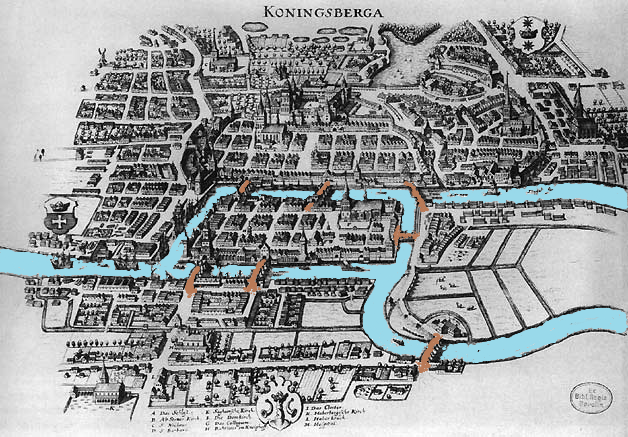
\includegraphics{koenigsberg_map_by_merian-erben_16521.png}}
  \vfill
  {\Large Jason D. Underdown}\\[\baselineskip]
  {
\includegraphics[scale=0.35]{slcc-logo}}\\[\baselineskip]
  {\large \today\ at \DTMcurrenttime{} }\\
\end{titlepage}

%%% Local Variables:
%%% mode: latex
%%% TeX-master: "Notes"
%%% End:

%%%%%%%%%%%%%%%%%%%%%%%%%%%%%% Copyright Page %%%%%%%%%%%%%%%%%%%%%%%%%%%%%%
{\noindent
  Copyright \copyright{}
  \hspace{0.2em} 2021
  \hspace{0.5em} Jason D. Underdown}
\doclicenseThis{}
\frontmatter{}
\pagestyle{plain}
%%%%%%%%%%%%%%%%%%%%%%%%%%%%%% Table of Contents %%%%%%%%%%%%%%%%%%%%%%%%%%%
\tableofcontents
\pagebreak
%%%%%%%%%%%%%%%%%%%%%%%%%%%%%% List of Theorems %%%%%%%%%%%%%%%%%%%%%%%%%%%%
\addcontentsline{toc}{chapter}{List of Theorems}
{\noindent \huge \textbf{List of Theorems}}
\vspace{0.5in}
\listtheorems{theorem}
%%%%%%%%%%%%%%%%%%%%%%%%%%%%%% Main Chapters %%%%%%%%%%%%%%%%%%%%%%%%%%%%%%%
\mainmatter{}
\pagestyle{myfancypage}
\chapter{Problem Solving}%
\label{chap:problem-solving}

\section{Exploiting Fractions for Fun and Profit}
\label{sec:proportions-rates}

\subsection{Absolute and Relative Change}
\label{sub:absolute-relative-change}

In this section we will see how to use the two arithemtic operations
of subtraction and division to measure how something changes over
time.
\begin{definition}
  \textbf{Absolute change} is the difference:
  \[
    \text{absolute change} = \text{new} - \text{old}
  \]
\end{definition}

Absolute change can be useful for comparing things that are similar.
For example you could compare how many inches two fourteen year old
boys grew in one year. But suppose the things you wish to compare are
related but on very different size scales.

\begin{example}[Stock Investments Part I]
  Suppose you invest \$50,000 in Acme corporation stock and after one
  year the stock is now worth \$52,000. This is an absolute change of
  \$2,000. Now suppose you also invest \$500 in Hooli corporation and
  after one year the stock is worth \$550. Which investment was better?
\end{example}
\begin{solution}
  \begin{align*}
    \text{absolute change in Acme} &= \$52,000 - \$50,000 = \$2,000 \\
    \text{absolute change in Hooli} &= \$550 - \$500 = \$50
  \end{align*}
  In terms of absolute change the yield from the Acme investment is
  larger, so it is better right? Well what if we had switched our
  investment strategy and swapped the initial stock purchase for each
  company? To answer this question we need to see how big the absolute
  change in value was relative to the initial outlay of money. We need
  relative change.
\end{solution}

\begin{definition}
  \textbf{Relative change} is the ratio of absolute change to the original (old) value.
  \[
    \text{relative change} = \frac{\text{new} - \text{old}}{\text{old}}
  \]
\end{definition}

\begin{example}[Stock Investments Part II]
What is the relative change in value of each stock purchase?
\end{example}
\begin{solution}
  \begin{align*}
    \text{relative change in Acme}
    &= \frac{\$52,000 - \$50,000}{\$50,000} = \frac{\$2,000}{\$50,000} = 0.04 \\
    \text{relative change in Hooli}
    &= \frac{\$550 - \$500}{\$500} = \frac{\$50}{\$500} = 0.10
  \end{align*}
  Hooli's relative change was higher than Acme's relative change, and
  thus the Hooli stock was the better investment.
\end{solution}

\begin{note}
  Notice that absolute change has units attached to the value. In the
  above examples the units were dollars (\$). But when you compute
  relative change, the numerator and denominator will have the same
  units and thus the units will cancel and you are left with a pure
  (unitless) number.
\end{note}

\subsection{Percentages}
\label{sub:percentages}

\begin{definition}
  A \textbf{percent} or \textbf{percentage} is a fraction, where the
  denominator is 100, but for ease of writing we drop the denominator
  and replace it with the percent symbol \(\%\). For example,
  \[
    \frac{3}{4} = 0.75 = \frac{75}{100} = 75\%
  \]
  Percentages can be negative and even larger than 100, for example
  \[
    250\% = \frac{250}{100} = 2.5
  \]
\end{definition}

\begin{exercise}
  Express the following values as percentages.
  \begin{enumerate}
  \item \(\displaystyle\frac{1}{5}\)
    \vspace*{\stretch{1}}
  \item \(\displaystyle 0.004\)
    \vspace*{\stretch{1}}
  \item \(\displaystyle 3.11\)
    \vspace*{\stretch{1}}
  \end{enumerate}
\end{exercise}

It is often convenient to express relative change as a percent
\begin{example}[Stock Investments Part III]
  What was the percent change in value of each stock investment?
  \begin{center}
    \begin{tabular}{rccc}
      \toprule
      Company & Decimal & Fraction & Percent \\
      \midrule
      Acme & .04 & \(\frac{4}{100}\) & 4\% \\ \\
      Hooli & .10 & \(\frac{10}{100}\) & 10\% \\
      \bottomrule
    \end{tabular}
\end{center}
\end{example}

\newpage

\begin{exercise}
  Your truck was worth \$28,000 in 2019 and is now worth \$23,500 in
  2021. What is the percent change in value of your truck?

  \vspace*{\stretch{1}}
\end{exercise}


\begin{exercise}
  Your \$290,000 home increased in value by 5\%. How much is it worth now?

  \vspace*{\stretch{1}}
\end{exercise}

\begin{exercise}
  A store has a clearance rack where every item is marked down 20\%
  off the original price. They have a sale advertising an additional
  20\% off everything in the store. What percentage of the original
  price do you end up paying?

  \vspace*{\stretch{1}}
\end{exercise}

\newpage

\subsection{Rates}
\label{sub:rates}

\begin{definition}
  A \text{rate} is a ratio of two quantities. Rates are also known as
  fractions.
\end{definition}

\begin{exercise}
  If your car can travel \US{284}{\mile} per fillup and your gas tank
  holds \US{9.5}{\gallon}, then at what rate does your car consume
  gasoline, or more commonly, what is its mpg?

  \vspace*{\stretch{1}}
\end{exercise}

\subsection{Proportionality}
\label{sub:proportionality}

\begin{definition}
  A \text{proportion} is a ratio of two quantities. Thus it is a fraction.
\end{definition}

\begin{exercise}
  A map's legend indicates that \US{0.5}{\inch} equals
  \US{4}{\mile}. How many miles apart in real life are two points on
  the map that are separated by \US{3.5}{\inch}?

  \vspace*{\stretch{1}}
\end{exercise}

\begin{exercise}
  A cookie recipe calls for 2 cups of chocolate chips per batch of 24
  cookies. If you wish to make 216 cookies?

  \vspace*{\stretch{1}}
\end{exercise}

\newpage

\section{Exploiting Units for Fun and Profit}
\label{sec:exploiting-units}

\begin{exercise}
  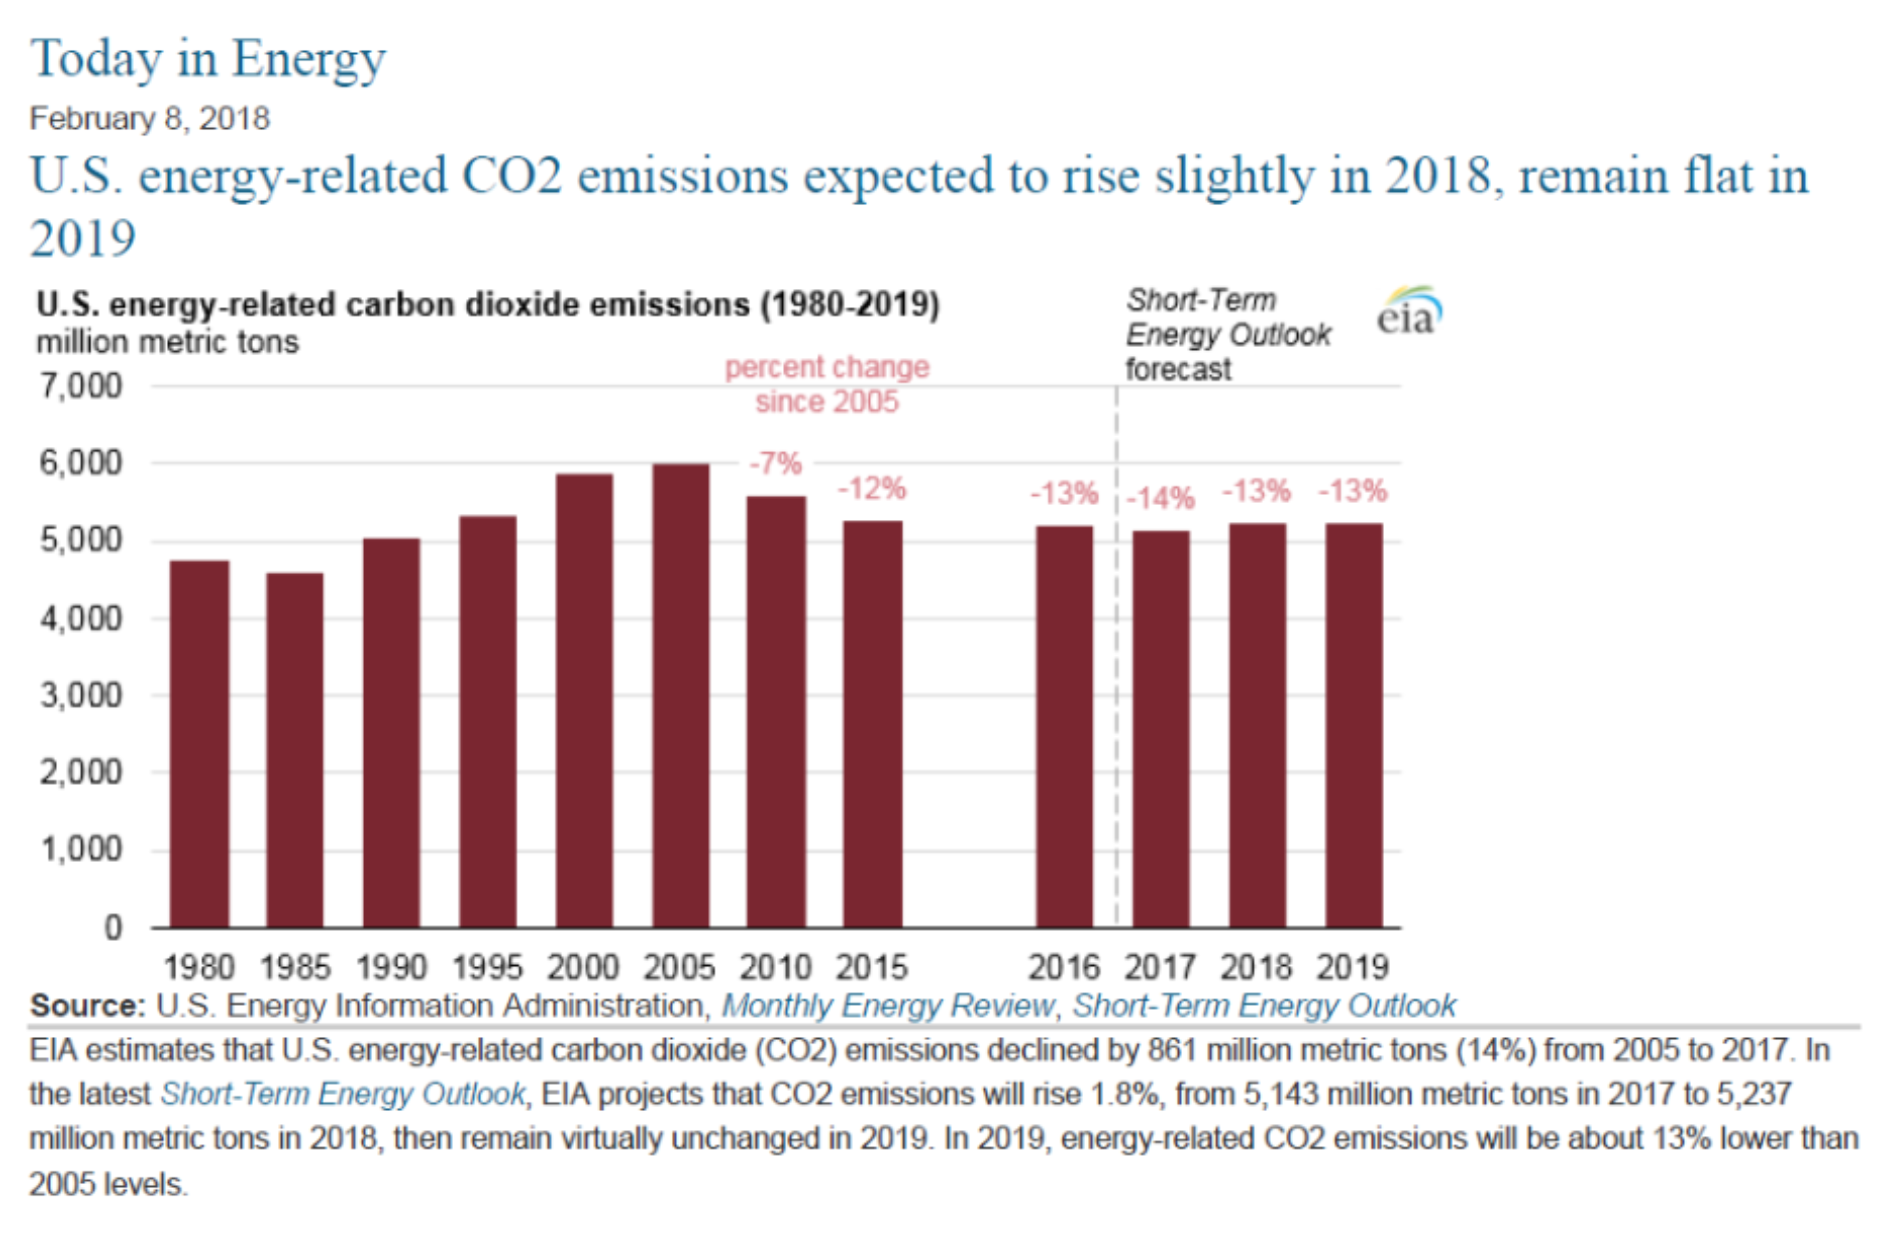
\includegraphics[scale=0.5]{CO2_Emissions}
  \begin{enumerate}
  \item According to EIA how much carbon did the American energy
    sector emit in 2017? How much is it predicted to emit in 2018 and
    2019?

    \vspace*{\stretch{1}}

  \item Use the absolute change from 2005 to 2017 given in the first
    sentence to calculated U.S. energy-related emissions in 2005.

    \vspace*{\stretch{1}}

  \item Use the result from part 2 to calculate the relative change
    from 2005 to 2017. Does your value agree with the given
    percentage?

    \vspace*{\stretch{1}}

    \newpage

    \begin{center}
      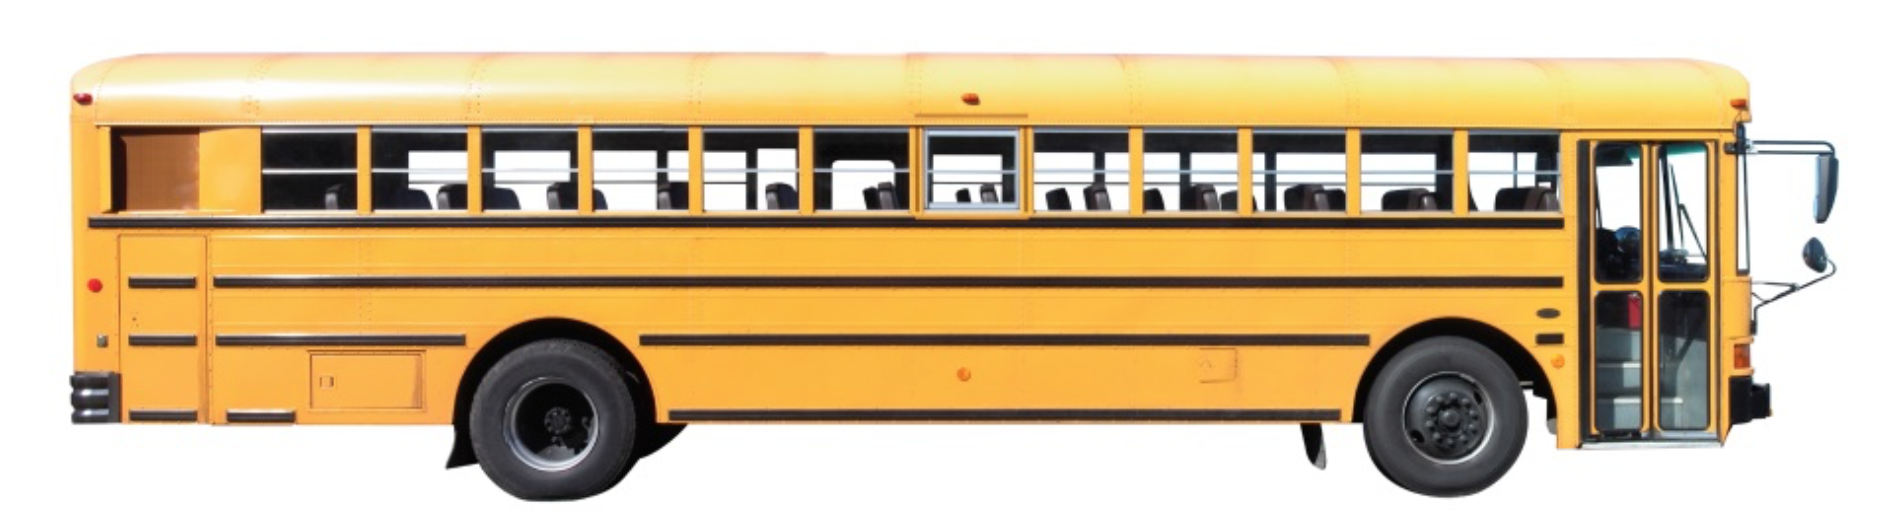
\includegraphics[scale=0.2]{schoolbus}
    \end{center}
  \item A Type D school bus weighs about 15 metric tons. How many
    school buses worth of \(\text{CO}_2\) did the American energy
    industry emit in 2005?
    \vspace*{\stretch{1}}

  \item How many school buses worth of \(\text{CO}_2\) is the American
    energy industry predicted to emit in 2019?

    \vspace*{\stretch{1}}


  \item According to the American School Bus Council about 480,000
    buses are used each day in the United States. Compare the weight
    of all those buses to the weight of the \(\text{CO}_2\) the U.S.
    energy sector is predicted to emit in 2019.

    \vspace*{\stretch{1}}
  \end{enumerate}
\end{exercise}

\newpage

\subsection{Unit Conversions}%
\label{sub:unit-conversions}

\begin{table}[h]
  \centering
  \begin{tabular}{lr@{ = }l}
    \toprule
    Length & 12 in & 1 ft \\
           & 3 ft & 1 yd \\
           & 5280 ft & 1 mi \\
    \midrule
    Weight & 1 lb & 16 oz \\
           & 1 ton & 2000 lb \\
    \midrule
    Capacity & 1 fl oz & \(\tfrac{1}{8}\) cup \\
           & 1 cup & 8 fl oz \\
           & 1 pint & 16 fl oz (2 cups) \\
           & 1 quart & 32 fl oz (4 cups) \\
           & 1 gallon & 128 fl oz (4 quarts) \\
    \bottomrule
  \end{tabular}
  \caption{Common US unit conversions}%
  \label{tab:unit-conversions}
\end{table}

\begin{exercise}
  Convert 5 cubic yards to cubic feet.

  \vspace*{\stretch{1}}
\end{exercise}

\newpage

\begin{exercise}
  During a massive Canadian ice storm, 30 thousand acres of sugarbush
  crop were damaged, where each acre of sugarbush grows about 80
  trees. You can assume that each tree yields \(\tfrac{1}{2}\) gallon
  of maple syrup a year, and Canada typically produces 8 million
  gallons of maple syrup per year.

  \begin{enumerate}
  \item What percentage of the maple syrup supply in Canada was destroyed
    that year?

    \vspace*{\stretch{1}}

  \item If maple syrup is worth \$39.10 per gallon and the average
    farmer tends to 45 acres of sugarbush, how much income did the
    average farmer lose that year?

    \vspace*{\stretch{1}}

  \end{enumerate}
\end{exercise}

\newpage

\subsection{Working In the Yard}%
\label{sub:working-in-yard}

\begin{figure}[h]
  \centering
  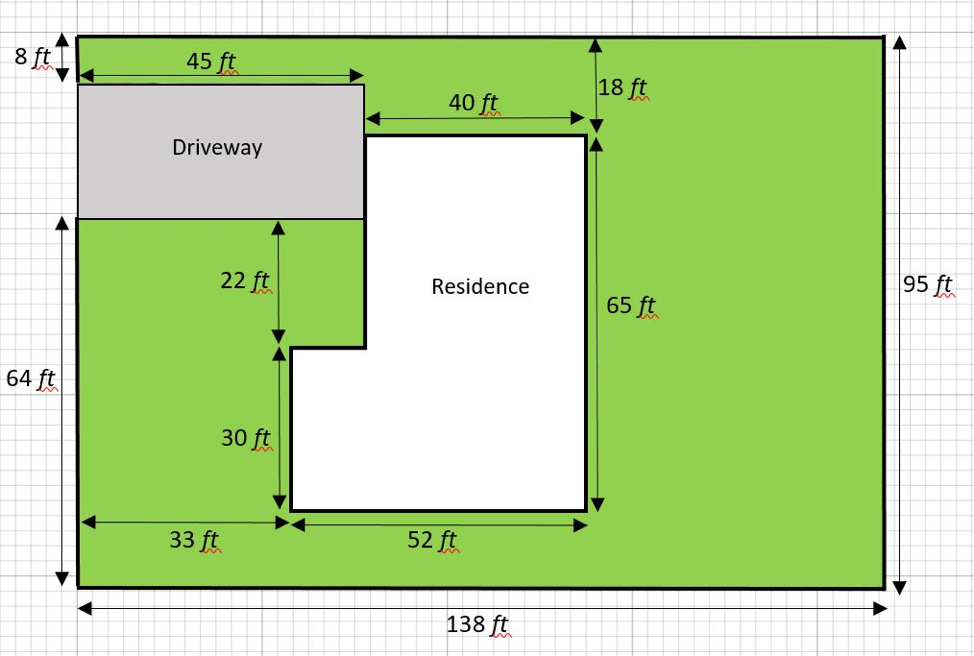
\includegraphics[width=\textwidth]{yard-schematic}
  \caption{Schematic of a plot of land.}%
  \label{fig:yard-schematic}
\end{figure}

\begin{exercise}
  Your neighbor's lawn isn't looking too good. He has decided to
  remove all the old sod (grass), bring in a new 4 inch layer of
  topsoil, install new in-ground sprinklers, and reseed the lawn. He
  seems to think that he'll be able to save money by hauling loads of
  topsoil from the store himself in his pickup truck, rather than
  paying for delivery, but you're not sure he's right. You're going to
  help him.
  \begin{enumerate}
  \item Using Figure~\ref{fig:yard-schematic}, find the area of the
    yard via the following steps:
    \begin{enumerate}
    \item Find the area of the entire lot.

      \vspace*{\stretch{1}}

    \item Find the area of the residence.

      \vspace*{\stretch{1}}

    \item Find the area of the driveway.

      \vspace*{\stretch{1}}

    \item Find the area of the yard.
    \end{enumerate}

    \newpage

  \item We are supposed to put a 4 inch layer of topsoil over the area
    of the yard.

    \begin{enumerate}
    \item Find the required topsoil in cubic feet.

      \vspace*{\stretch{1}}

    \item Convert the required volume of topsoil to cubic yards.

      \vspace*{\stretch{1}}

    \item Find the cost of the topsoil. (\$18 per cubic yard sold in
      \(\tfrac{1}{4}\) cubic yard increments)

      \vspace*{\stretch{1}}
    \end{enumerate}

  \item Suppose we pay \$30 per truckload on top of the soil cost.
    Each truckload can deliver up to 18 cubic yards.
    \begin{enumerate}
    \item How many truckloads are required?

      \vspace*{\stretch{1}}

    \item How much will the delivery cost?

      \vspace*{\stretch{1}}

    \end{enumerate}

    \newpage

  \item Suppose we use the pickup truck. The bed is 80 inches long, 69
    inches wide, and 20 inches tall.
    \begin{enumerate}
    \item Calculate the volume of the pickup in cubic inches.

      \vspace*{\stretch{1}}

    \item Convert the volume of the pickup to cubic yards.

      \vspace*{\stretch{1}}

    \item How many trips to the store will we need to make?

      \vspace*{\stretch{1}}

    \item The store is 9 miles away and it takes 20 minutes to drive
      there. The truck gets 17 miles to the gallon and gasoline costs
      \$3.79 per gallon. How much will we pay to get the soil
      ourselves?

      \vspace*{\stretch{1}}

    \item How much time will we spend driving?
    \end{enumerate}

      \vspace*{\stretch{1}}

  \end{enumerate}
\end{exercise}



% \subsection{Geometry: Area and Volume Formulas}
% \label{sub:geometry}


% \subsection{Linear, Areal and Volumetric Densities}
% \label{sub:densities}





%%% Local Variables:
%%% mode: latex
%%% TeX-master: "Notes"
%%% End:

\include{measurement}
\chapter{Voting Theory}%
\label{chap:voting-theory}

In many decision making situations, it is necessary to gather the
group consensus. This happens when a group of friends decides which
movie to watch, when a company decides which product design to
manufacture, and when a democratic country elects its leaders.

While the basic idea of voting is fairly universal, the method by
which those votes are used to determine a winner can vary. Amongst a
group of friends, you may decide upon a movie by voting for all the
movies you're willing to watch, with the winner being the one with the
greatest approval. A company might eliminate unpopular designs then
revote on the remaining. A country might look for the candidate with
the most votes.

In deciding upon a winner, there is always one main goal: to reflect
the preferences of the people in the most fair way possible. However,
we will see that there is more than one criteria for fairness. In
fact, there are several different criteria which can be used to
determine whether an election or decision process is fair or not.

In this chapter we will look at several methods for a group to make a
choice and analyze each method's strengths and weaknesses.

\section{Plurality Voting Method}%
\label{sec:plurality-method}

In the United States, most elections choose the winner based upon
which ever candidate receives the most votes. Notice that it is
\emph{not} necessary to receive a \emph{majority} (more than half) of
the votes, just more votes than any other candidate.

\begin{definition}
  The \textbf{plurality} voting method chooses the winner based on the
  candidate which receives more votes than any other candidate.
\end{definition}

\newpage

\begin{exercise}
  If Alex, Betty and Chuck are running for the office of club
  president, then what is the minimum number of votes that one could
  get to win the election under the plurality method if there are
  \begin{enumerate}
  \item 73 votes cast?
    \vspace*{\stretch{1}}
  \item 74 votes cast?
    \vspace*{\stretch{1}}
  \end{enumerate}
\end{exercise}

A two-party system often develops in a plurality voting system. In
this system, voters have a single vote, which they can cast for a
single candidate in their district, in which only one legislative seat
is available. In plurality voting (also referred to as
\textbf{first-past-the-post}), in which the winner of the seat is
determined purely by the candidate with the most votes, several
characteristics can serve to discourage the development of third
parties and reward the two major parties.

Because the first-past-the-post system gives only the (plurality)
winner in each district a seat, a party that consistently comes in
second or third in many or most districts will not gain any seats in
the legislature, even if it receives a substantial minority of the
vote.

Another challenge to a third party is both statistical and tactical.
Political scientist Maurice Duverger presents the example of an
election in which 100,000 moderate voters and 80,000 radical voters
are to vote for candidates for a single seat or office. If two
moderate parties ran candidates and one radical candidate ran (and
every voter voted), the radical candidate would tend to win unless one
of the moderate candidates gathered fewer than 20,000 votes.
Appreciating this risk, moderate voters would be inclined to vote for
the moderate candidate they deemed likely to gain more votes, with the
goal of defeating the radical candidate. To win, then, either the two
moderate parties must merge, or one moderate party must fail, as the
voters gravitate to the two strongest parties. Duverger called this
trend polarization.

\section{Instant Runoff Voting (Ranked Choice Voting)}%
\label{sec:irv}

What if we required the eventual winner to receive a \emph{majority}
in order to win? This may not be possible if there are more than two
candidates. A way around this problem is to do \textbf{runoff voting}
where the election is held in stages. After each vote, if a single
candidate has a majority of the votes then that candidate wins, but if
not, then the candidate with the least votes is eliminated and
everyone votes again. Clearly this is time consuming and inefficient.
One way around the inefficiencey of runoff voting is to modify the
ballot to allow voters to rank the candidates by order of preference.

\begin{definition}\label{def:preference-ballot-schedule}
  A \textbf{preference ballot} is a ballot in which the voter ranks
  the choices in order of preference.

  Once the election has been held we tally the votes and create a
  summary of voter preferences. We call this summary of the ballots a
  \textbf{preference schedule}.
\end{definition}

\begin{exercise}
  Below is an example of a preference schedule for candidates A,B,C and D.
  \begin{table}[h]
    \centering
    \begin{tabular}{ccccc}
      \toprule
      Num. Ballots & 8 & 17 & 4 & 11 \\
      \midrule
      1st & A & D & B & C \\
      2nd & B & A & A & B \\
      3rd & C & C & D & A \\
      4th & D & B & C & D \\
      \bottomrule
    \end{tabular}
    \caption{Example preference schedule}%
    \label{tab:example-preference-schedule}
  \end{table}
  Notice that there were a total of \( 8+17+4+11=40 \) votes cast.
  This means that for a candidate to get a \emph{majority} of the
  votes they must get at least 21 votes because 21 is the smallest
  whole number that is more than half of 40.

  \begin{enumerate}
  \item Who wins under the plurality method?

    \vspace*{\stretch{1}}

  \item Who is the winner under instant-runoff voting?

    \vspace*{\stretch{5}}

  \end{enumerate}
\end{exercise}

\newpage

\begin{exercise}
  Suppose there is an election with four candidates. Two are from the
  two dominant political parties: Democrat and Republican. The other
  two are from third parties: Libertarian and Socialist. A preference
  schedule is given below.
  \begin{center}
    \begin{tabular}{ccccc}
      \toprule
      Num. Ballots & 8 & 18 & 20 & 4 \\
      \midrule
      1st & L & R & D & S \\
      2nd & R & L & S & D \\
      3rd & D & S & L & R \\
      4th & S & D & R & L \\
      \bottomrule
    \end{tabular}
  \end{center}
  Answer the following questions using the data in the preference
  schedule above.
  \begin{enumerate}
  \item How many people voted?

    \vspace*{\stretch{1}}

  \item How many votes are required for a majority?

    \vspace*{\stretch{1}}

  \item What is the smallest possible number of votes a candidate
    could win with under the plurality method of choosing?

    \vspace*{\stretch{1}}


  \item Who wins under instant runoff voting?
    \vspace*{\stretch{5}}

  \end{enumerate}
\end{exercise}

\newpage

\section{Borda Count}%
\label{sec:borda-count}

Borda Count is another voting method, named for Jean-Charles de Borda,
who developed the system in 1770.

\begin{definition}
  In the \textbf{Borda Count} method, points are assigned to
  candidates based on their ranking; 1 point for last choice, 2 points
  for second-to-last choice, and so on. The point values for all
  ballots are totaled, and the candidate with the largest point total
  is the winner.
\end{definition}

\begin{exercise}\label{ex:borda-count}
  Suppose an election resulted in the following preference schedule.
  Which of the three candidates: A, B, or C would win under the Borda
  count method of choosing?
  \begin{center}
    \begin{tabular}{ccccc}
      \toprule
      Num. Ballots & 13 & 4 & 14 \\
      \midrule
      1st & B & A & C \\
      2nd & A & B & A \\
      3rd & C & C & B \\
      \bottomrule
    \end{tabular}
  \end{center}

  \vspace*{\stretch{1}}
\end{exercise}

\begin{exercise}\label{ex:irv}
  Which candidate would win under instant runoff voting?

  \vspace*{\stretch{1}}
\end{exercise}

\newpage

\section{Copeland's Method (Pairwise Comparison)}%
\label{sec:copelands-method}

Sometimes a candidate can be preferred by voters when compared to
every other candidate, but still not win the election. This seems
unfair to most people.

\begin{definition}
  If one candidate is preferable to all other candidates in
  head-to-head matchups, then that candidate is called the
  \textbf{Condorcet candidate}.
\end{definition}

\begin{exercise}\label{ex:copeland}
  Use the preference schedule from exercise~\ref{ex:borda-count} to
  determine if there was a Condorcet candidate in that election. The
  table is reproduced below.
  \begin{center}
    \begin{tabular}{ccccc}
      \toprule
      Num. Ballots & 13 & 4 & 14 \\
      \midrule
      1st & B & A & C \\
      2nd & A & B & A \\
      3rd & C & C & B \\
      \bottomrule
    \end{tabular}
  \end{center}

  \vspace*{\stretch{1}}
\end{exercise}



\section{Fairness Criteria}%
\label{sec:fairness criteria}

\begin{definition}
  A \textbf{fairness criterion} is a conditional statement (if---then)
  about a selection or voting method that seems like it should be
  satisfied in order for the method to be fair.
\end{definition}

\begin{description}
\item[Plurality Criterion] \hfill \\
  If there is a candidate that gets more votes than any other
  candidate, then that candidate should win.
\item[Majority Criterion] \hfill \\
  If there is a candidate that has a majority (more than half) of
  first-place votes, then that candidate should win.
\item[Condorcet Criterion] \hfill \\
  If there is a candidate that wins every head-to-head comparison,
  then that candidate should win.
\item[Monotonicity Criterion] \hfill \\
  If a candidate wins, and only changes that favor the winner are made
  to the preference ballots, then that candidate should still win.
\item[Independence of Irrelevant Alternatives (IIA) Criterion] \hfill \\
  If a candidate wins, and only losing candidates are removed from the
  preference ballots, then that candidate should still win.
\end{description}


\section{Arrow's Impossibility Theorem}%
\label{sec:arrows-impossibility-thm}





%%% Local Variables:
%%% mode: latex
%%% TeX-master: "Notes"
%%% End:

\chapter{Graph Theory}%
\label{chap:graph-theory}

\section{Vocabulary}%
\label{sec:vocabulary}

\begin{definition}
  A \textbf{vertex} is a dot or circle, often labelled with a letter
  or short name. An edge is a line or arc which connects two
  \textbf{vertices}. A \textbf{loop} is a special kind of edge that
  connects a vertex to itself.
\end{definition}

\begin{definition}
  A \textbf{graph} is a pair of sets, a set of \textbf{vertices}, and
  a set of \textbf{edges}.
\end{definition}

\begin{definition}
  The \textbf{degree} of a vertex is the number of edges meeting at
  that vertex.
\end{definition}

\begin{definition}
  A \textbf{path} is an ordered sequence of edges.
\end{definition}
\begin{note}
  For brevity we sometimes denote a path as a sequence of vertices.
\end{note}

\begin{definition}
  A \textbf{circuit} is a path that begins and ends at the same
  vertex.
\end{definition}

\begin{definition}
  A graph is \textbf{connected} if there is a path from any vertex to
  any other vertex.
\end{definition}

\begin{definition}
  A \textbf{weighted graph} is a graph where each edge has a numerical
  value associated with it. The weights often correspond with
  distances, travel time, or travel cost.
\end{definition}

\section{Dijkstra's Algorithm (Shortest Path)}%
\label{sec:dijkstras-algorithm}

\begin{algorithm}[Dijkstra's Algorithm]
  \begin{enumerate}
  \item Mark the ending vertex with a distance of zero. Designate this
    vertex as current.

  \item Find all vertices leading to the current vertex. Calculate
    their distances to the end. Since we already know the distance the
    current vertex is from the end, this will just require adding the
    most recent edge. Don't record this distance if it is longer than
    a previously recorded distance.

  \item Mark the current vertex as visited. We will never look at this
    vertex again.

  \item Mark the vertex with the smallest distance as current, and
    repeat from step 2.
  \end{enumerate}
\end{algorithm}

\section{Eulerian Circuits and the Chinese Postman Problem}%
\label{sec:eulerian-circuits}

\subsection{Fleury's Algorithm}%
\label{sub:Fleury's Algorithm}

\begin{algorithm}[Chinese Postman --- Fleury]
  \begin{enumerate}
  \item Start at any vertex if finding an Euler circuit. If finding an
    Euler path, start at one of the two vertices with odd degree.
  \item Choose any edge leaving your current vertex, provided deleting
    that edge will not separate the graph into two disconnected sets
    of edges.
  \item Add that edge to your circuit, and delete it from the graph.
  \item Continue until you're done.
  \end{enumerate}
\end{algorithm}

\section{Hamiltonian Circuits and the Traveling Salesman Problem}%
\label{sec:hamiltonian-circuits}

\subsection{Brute Force}%
\label{sub:brute-force}

\begin{algorithm}[Brute Force]
  \begin{enumerate}
  \item Create a list of all possible circuits and their costs.
  \item Choose the circuit with the least cost.
  \end{enumerate}
\end{algorithm}

\subsection{Nearest Neighbor Algorithm (NNA)}%
\label{sub:nearest-neighbor}

\begin{algorithm}[Nearest Neighbor Algorithm]
  \begin{enumerate}
  \item Select a starting point.
  \item Move to the nearest unvisited vertex (via the edge with
    smallest weight).
  \item Repeat until the circuit is complete.
  \end{enumerate}
\end{algorithm}

\subsection{Repeated Nearest Neighbor Algorithm (RNNA)}%
\label{sub:repeated-nearest-neighbor}

\begin{algorithm}[Repeated Nearest Neighbor Algorithm]
  \begin{enumerate}
  \item Do the Nearest Neighbor Algorithm starting at each vertex.
  \item Choose the circuit produced with minimal total weight.
  \end{enumerate}
\end{algorithm}

\subsection{Sorted Edges Algorithm (SEA)}%
\label{sub:sorted-edges}

\begin{algorithm}[Sorted Edges Algorithm]
  \begin{enumerate}
  \item Select the cheapest unused edge in the graph.
  \item Repeat step 1, adding the cheapest unused edge to the circuit,
    unless:
    \begin{enumerate}
    \item adding the edge would create a circuit that doesn't contain
      all vertices, or
    \item adding the edge would give a vertex degree 3.
    \end{enumerate}
  \item Repeat until a circuit containing all vertices is formed.
  \end{enumerate}
\end{algorithm}

\section{Spanning Trees and Kruskal's Algorithm}%
\label{sec:spanning-trees}



%%% Local Variables:
%%% mode: latex
%%% TeX-master: "Notes"
%%% End:

\chapter{Growth Models}%
\label{chap:growth-models}

\begin{definition}
  A \textbf{recursive} function is a function defined in terms of its
  previous value(s).
\end{definition}

\begin{note}
  A recursive function is easy to define, but hard to evaluate because
  you have to compute all the previous values.
\end{note}

\begin{example}[Fibonacci Sequence]
  The famous Fibonacci function is defined recursively as follows:
  \[
    F(x+2) = F(x)+F(x+1).
  \]
  Defining \(F(0)=0\) and \(F(1)=1\) yields the following sequence of
  outputs:
  \begin{align*}
    F(0) &= 0 \\
    F(1) &= 1 \\
    F(2) &= F(0) + F(1) = 0+1 = 1 \\
    F(3) &= F(1) + F(2) = 1+1 = 2 \\
    F(4) &= F(2) + F(3) = 1+2 = 3 \\
    F(5) &= F(3) + F(4) = 2+3 = 5 \\
    F(6) &= F(4) + F(5) = 3+5 = 8 \\
    F(7) &= F(5) + F(6) = 5+8 = 13 \\
     & \: \: \: \vdots
  \end{align*}
  Each number in the sequence, is the sum of the previous two numbers:
  \(0, 1, 1, 2, 3, 5, 8, 13, 21, 34\ldots\)
\end{example}

\section{Linear Growth}%
\label{sec:linear-growth}

\subsection{Recursive Linear Growth Model}%
\label{sec:recursive-linear}

Let \(P=\) population, \(x=\) unit of time, then we can define next
years population, \(P(x+1)\) in terms of this years population,
\(P(x)\), plus a fixed amount, \(d\).

\begin{equation}
  \boxed{P(x+1) = P(x) + d}\label{eq:recursive-linear-model}
\end{equation}

Thus \textbf{linear growth} (or decay) is characterized by the
\emph{difference} between any two successive time periods being
constant: \(d\).
\[
  P(x+1) - P(x) = d
\]

\subsection{Explicit Linear Growth Model}%
\label{sec:explicit-linear}

Let \(P_0\equiv P(0)\), and recall the recursive definition:
\(P(x+1) = P(x) + d \)
\begin{align*}
  P(1) &= P_0 + d \\
  P(2) &= P(1) + d = (P_0 + d) + d = P_0 + 2d \\
  P(3) &= P(2) + d = (P_0 + 2d) + d = P_0 + 3d \\
  P(4) &= P(3) + d = (P_0 + 3d) + d = P_0 + 4d \\
       & \: \: \vdots \\
  P(x) &= P_0 + xd\\
  \intertext{Or equivalently,}
  \Aboxed{P(x) &= dx + P_0}
\end{align*}
where \(d\) is the slope or growth rate, and \(P_0\) is the
\(y\)--intercept, or initial population.

\section{Exponential Growth}%
\label{sec:exponential-growth}

\subsection{Recursive Exponential Growth Model}%
\label{sec:recursive-exponential}


\subsection{Explicit Exponential Growth Model}%
\label{sec:explicit-exponential}

\subsection{Logarithms}%
\label{sec:logarithms}


\section{Logistic Growth}%
\label{sec:logistic-growth}

\section{Summary}%
\label{sec:growth-models-summary}






%%% Local Variables:
%%% mode: latex
%%% TeX-master: "Notes"
%%% End:

\chapter{Finance}%
\label{chap:finance}

\section{Simple Interest}%
\label{sec:simple-interest}


\begin{definition}
  \textbf{Simple interest} refers to a one-time interest payment.
  Simple interest is used for short-term loans.
  \begin{align}
    I &= rP_{0} \notag \\
    A &= P_{0} + I \notag \\
    A &= P_{0} + rP_{0} \notag \\
    \Aboxed{A &= P_{0}(1+r)} \label{eq:simple-interest}
    \intertext{where,}
    I &= \text{ interest} \notag \\
    A &= \text{ account balance (amount in the account)} \notag \\
    P_{0} &= \text{ principal (starting amount)} \notag \\
    r &= \text{ interest rate (in decimal)} \notag
  \end{align}
\end{definition}

\begin{exercise}
  A friend agrees to loan you \$500 to help you buy a new laptop. You
  agree to pay them back in 30 days with 3\% interest. How much will
  you owe your friend in 30 days?

  \vspace*{\stretch{1}}
\end{exercise}

\newpage
\section{Simple Interest Over Time}%
\label{sec:simple-interest}


\begin{definition}
  \textbf{Simple interest over time} refers to a fixed interest
  payment that accrues once each year. Simple interest is used for
  bonds. A \textbf{bond} is a loan that you make to the government.
  All levels of government issue bonds; municipal, state and federal.

  \medskip

  \noindent When you purchase a bond, the government agrees to pay you a fixed
  interest payment each year until the bond \emph{matures} whereupon
  they return the initial amount they borrowed from you. A bond
  matures after a fixed number of years, often 5, 10, 20 or 30 years.

  \begin{align}
    I &= rP_{0}n \notag \\
    A_{n} &= P_{0} + I \notag \\
    A_{n} &= P_{0} + rP_{0}n \notag \\
    \Aboxed{A_{n} &= P_{0}(1+rn)} \label{eq:bond-interest}
    \intertext{where,}
    I &= \text{ interest} \notag \\
    A_{n} &= \text{ account balance (amount in the account)} \notag \\
    P_{0} &= \text{ principal (starting amount)} \notag \\
    r &= \text{ interest rate (in decimal)} \notag \\
    n &= \text{ time (in years)} \notag
  \end{align}
\end{definition}
\begin{note}
  Simple interest over time corresponds with \emph{linear growth}.
  \begin{align*}
    f(x) &= mx + b, \\
    A_{n} &= (rP_{0})n + P_{0},
  \end{align*}
  where \(rP_{0}\) is the slope (or fixed amount of yearly increase),
  and \(P_{0}\) is the \(y\)-intercept.
\end{note}

\begin{exercise}
  Suppose you buy a municipal bond from your local city government to
  help fund construction projects at the local zoo. The bond costs
  \$2000, pays 2.5\% interest annually and matures in 10 years. How
  much interest will you earn?

  \vspace*{\stretch{1}}
\end{exercise}

\newpage

\section{Compound Interest}%
\label{sec:compound-interest}

\begin{definition}
  \textbf{Compound interest} refers to any situation where prior
  interest payments also accrue interest.
  \begin{align}
    \Aboxed{A_{n}&= P_{0} {\left( 1+\frac{r}{k} \right)}^{nk}}
      \label{eq:compound-interest}\\
    \intertext{where,}
    A_{n} &= \text{ account balance after } n \text{ years.} \notag \\
    P_{0} &= \text{ principal (starting amount)} \notag \\
    r &= \text{ annual interest rate (in decimal)} \notag \\
    k &= \text{ the number of compounding periods per year} \notag
  \end{align}
\end{definition}
\begin{note}
  If \(k=1\), \ie{} there is only one compounding per year then the
  formula becomes
  \[
    \boxed{A_{n} = P_{0}{(1+r)}^{n},}
  \]
  which is the \emph{exponential population model}.
\end{note}

\begin{exercise}
  Suppose you deposit \$1000 into a bank account which earns 3\%
  interest compounded monthly. How much money will you have after one
  year?

  \vspace*{\stretch{1}}
  \noindent Answer: \$1,030.42
\end{exercise}

\newpage

\begin{exercise}
  A certificate of deposit (CD) is a savings instrument that many
  banks offer. It usually gives a higher interest rate, but you cannot
  access your investment for a specified length of time. Suppose you
  deposit \$3000 in a CD paying 6\% interest, compounded monthly. How
  much will you have in the account after 20 years?

  \vspace*{\stretch{1}}
  \noindent Answer: \$9,930.61
\end{exercise}

\begin{exercise}
  Again suppose you purchase a CD that pays 6\% interest compounded
  monthly. How long will it take for your initial deposit (the
  principal, \(P_{0}\)) to double?

  \medskip

  \noindent\emph{Hint: You don't need to know the principal, just use
    the symbol \(P_{0}\).}

  \vspace*{\stretch{1}}
\end{exercise}

\newpage

\section{Saving Annuities}%
\label{sec:annuities}

\begin{definition}
  A \textbf{savings annuity} is an account into which regular payments
  are made for a fixed number of years. When the annuity matures you
  receive the payments and the interest that each payment accrued.

  \begin{align}
    \Aboxed{A_{n}
    &= \frac{d\left[ {\left( 1+\frac{r}{k} \right)}^{nk} - 1 \right]}
      {\left( \frac{r}{k} \right)}} \\
    \intertext{where,}
    A_{n} &= \text{ account balance after } n \text{ years.} \notag \\
    d &= \text{ regular deposit} \notag \\
    r &= \text{ annual interest rate (in decimal)} \notag \\
    k &= \text{ the number of compounding periods per year} \notag
  \end{align}
\end{definition}

\begin{exercise}
  At the age of 30, Susan, opens a savings annuity account that pays
  6\% interest compounded monthly. She agrees to make a deposit of
  \$200 every month for 35 years. How much will the annuity be worth
  after 35 years when she is 65?

  \vspace*{\stretch{1}}
  \noindent Answer: \$284,000.06
\end{exercise}

\newpage

When retirement planning, the object is to determine how much you need
to save each month now in order to have a guaranteed fixed income
during your retirement years. This requires solving the savings
annuity formula for \(d\):

\begin{align}
  A_{n}
  &=\frac{d\left[ {\left( 1+\frac{r}{k} \right)}^{nk} - 1 \right]}
    {\left( \frac{r}{k} \right)} \notag \\
  A_{n}\left( \frac{r}{k} \right)
  &=d\left[ {\left( 1+\frac{r}{k} \right)}^{nk} - 1 \right] \notag \\
  \frac{A_{n}\left( \frac{r}{k} \right)}
  {\left[ {\left( 1+\frac{r}{k} \right)}^{nk} - 1 \right]}
  &=d \notag \\
  \Aboxed{d
  &=\frac
    {A_{n} \left( \frac{r}{k} \right)}
    {\left[ {\left( 1+\frac{r}{k} \right)}^{nk} - 1 \right]}}%
    \label{eq:savings-annuity-pmt}
\end{align}

\begin{exercise}
  Suppose you know that you are going to need \$400,000 when you
  retire. If you don't yet have any retirement savings, but you have
  35 years until you will retire, how much do you need to save each
  month into an annuity that pays 7\% interest compounded monthly to
  amass a \$400,000 nest egg?

  \vspace*{\stretch{1}}
  \noindent Answer: \$222.09
\end{exercise}

\newpage

\section{Payout Annuities}%
\label{sec:payout-annuities}

\begin{definition}
  A \textbf{payout annuity} is an account from which regular payments
  are made to you for a fixed number of years. After the fixed number
  of years, the annuity is worth nothing. Payout annuities are often
  used for retirement, payment of lottery winnings and payment of
  legal settlements.

  \begin{align}
    \Aboxed{P_{0}
    &= \frac{d\left[ {1 - \left( 1+\frac{r}{k} \right)}^{-nk} \right]}
      {\left( \frac{r}{k} \right)}} \label{eq:payout-annuity} \\
    \intertext{where,}
    P_{0} &= \text{Principal or starting balance} \notag \\
    d &= \text{ regular payment} \notag \\
    r &= \text{ annual interest rate (in decimal)} \notag \\
    k &= \text{ the number of compounding periods per year} \notag
  \end{align}
\end{definition}

\begin{exercise}
  In retirement, you determine that you will need \$2,500 per month
  for a total of 30 years. If the annuity earns 6\% interest, how much
  principal will you need to fund this retirement annuity? And how
  much will the annuity pay out over its lifetime?

  \vspace*{\stretch{1}}
  \noindent Answers: \$416,979.04, \$900,000.00
\end{exercise}

\newpage

\subsection{Retirement Planning}%
\label{sub:retirement-planning}

\begin{exercise}
  Suppose you are currently 25 years old, but you plan to begin saving
  for retirement at age 30 and you plan to retire at age 65. You
  determine that you would like to have \$4000 per month for 30 years.
  \begin{enumerate}
  \item How much principal will you need at age 65 to fund a payout
    annuity if the annuity yields 6\% interest?

    \vspace*{\stretch{3}}

  \item How much will you need to save each month beginning at age 30
    if your savings annuity yields 8\% interest?

    \vspace*{\stretch{3}}

  \item How much will you need to save each month if you begin saving
    for retirement at age 25 instead of 30, so you will have
    \(65-25=40\) total years of saving?

    \vspace*{\stretch{3}}

  \item How much money did you save for retirement? (Use calculation
    from question 3.)

    \vspace*{\stretch{1}}

  \item And how much money in total did you receive from that
    investment?

    \vspace*{\stretch{1}}

  \end{enumerate}

  \noindent Answers: (1) \$667,166.46, (2) \$290.85, (3) \$191.11,
  (4) \$91,732.80, (5) \$1,440,000.00
\end{exercise}

\newpage

\section{Loans}%
\label{sec:loans}

In this section, you will learn about conventional loans (also called
amortized loans or installment loans). Examples include auto loans and
home mortgages. These techniques do not apply to payday loans, add-on
loans, or other loan types where the interest is calculated up front.

One great thing about loans is that they use exactly the same formula
as a payout annuity. To see why, imagine that you had \$10,000
invested at a bank, and started taking out payments while earning
interest as part of a payout annuity, and after 5 years your balance
was zero. Flip that around, and imagine that you are acting as the
bank, and a car lender is acting as you. The car lender invests
\$10,000 in you. Since you're acting as the bank, you pay interest.
The car lender takes payments until the balance is zero.
\[
  \boxed{P_{0}
    = \frac{d\left[ {1 - \left( 1+\frac{r}{k} \right)}^{-nk} \right]}
    {\left( \frac{r}{k} \right)}}
\]
\begin{exercise}
  You can afford to pay \$280 per month for a car payment. If you
  qualify for an auto loan at 3\% interest for a term of 60 months (5
  years), how expensive of a car can you afford?

  \vspace*{\stretch{1}}
\end{exercise}

\noindent Answer: \$15,582.66

\newpage

Often when taking out a loan, you know the principal of the loan, but
you need to figure out what that amounts to in monthly payments. To do
this we can solve the payout annuity formula~\eqref{eq:payout-annuity}
for \(d\), the payment amount:

\begin{align*}
  P_{0}
  &= \frac{d\left[ {1 - \left( 1+\frac{r}{k} \right)}^{-nk} \right]}
    {\left( \frac{r}{k} \right)} \\
  P_{0}\left( \frac{r}{k} \right)
  &= d\left[ {1 - \left( 1+\frac{r}{k} \right)}^{-nk} \right] \\
  \frac{P_{0}\left( \frac{r}{k} \right)}
  {\left[ {1 - \left( 1+\frac{r}{k} \right)}^{-nk} \right]}
  &= d \\ \\
  \Aboxed{
  d &=
      \frac{P_{0}\left( \frac{r}{k} \right)}
      {\left[ {1 - \left( 1+\frac{r}{k} \right)}^{-nk} \right]}
  }
\end{align*}
\begin{exercise}
  You wish to take out a \$300,000 mortgage (home loan). If you
  qualify for a fixed interest rate of 4\% and you choose a 30 year
  term. How much will your monthly payments be?

  \vspace*{\stretch{1}}
\end{exercise}

\noindent Answer: \$1,432.25
\newpage

\section{Loan Payoff}%
\label{sec:loan-payoff}

To determine the remaining loan balance, we can think ``how much loan
will these loan payments be able to pay off in the remaining time on
the loan?''

\begin{note}
  Many people mistakenly believe that the payoff amount is simply
  their monthly payment times the number of remaining payments. This
  will always be more than the actual payoff amount.
\end{note}

\begin{exercise}
  Suppose you purchased your home with a 30 year mortgage for
  \$250,000 at a 3.5\% interest rate. Your monthly morgage payment is
  \$1122.61.

  \begin{enumerate}
  \item If you have made payments for 5 years (60 payments), what is
    the payoff amount? In other words how much money would you have to
    give the lender today to settle the mortgage debt?

    \vspace*{\stretch{3}}

  \item How much have you payed to the bank (mortgage lender) over
    five years?

    \vspace*{\stretch{1}}

  \item How much of the money you payed went towards interest?

    \vspace*{\stretch{1}}

  \end{enumerate}
\end{exercise}

\noindent Answers: (1) \$224,242.68, (2) \$67,356.60, (3) \$41,599.28

\newpage

\begin{exercise}
  Suppose your monthly car payment is \$366.

  \begin{enumerate}
  \item If your loan has a 5 year term and you have made payments for
    3 years (36 payments) what is your loan payoff amount?

    \vspace*{\stretch{1}}

  \item How much in total will you pay if you continue making payments
    for two years?

    \vspace*{\stretch{1}}

  \end{enumerate}
\end{exercise}


%%% Local Variables:
%%% mode: latex
%%% TeX-master: "Notes"
%%% End:

\chapter{Introduction to Statistics}%
\label{chap:intro-statistics}


%%% Local Variables:
%%% mode: latex
%%% TeX-master: "Notes"
%%% End:

\chapter{Describing Data}%
\label{chap:describing-data}


%%% Local Variables:
%%% mode: latex
%%% TeX-master: "Notes"
%%% End:

\chapter{Probability}%
\label{chap:probability}


%%% Local Variables:
%%% mode: latex
%%% TeX-master: "Notes"
%%% End:


%%%%%%%%%%%%%%%%%%%%%%%%%%%%%% Appendices %%%%%%%%%%%%%%%%%%%%%%%%%%%%%%%%%%
\pagestyle{plain}
% \begin{appendices}
%   \appendix
%   \noappendicestocpagenum{}
%   \addappheadtotoc{}
%   \chapter{Converse of the Pythagorean Theorem}%
\label{app:converse-pythagorean-thm}

This \href{http://jwilson.coe.uga.edu/EMAT6680/Brown/6690/ConPythagThm.htm}%
{proof} comes from Jim Wilson at the University of Georgia.

The proof uses a technique called \textbf{proof by contradiction}
which is a little tricky, thus it has been relegated to obscurity in
this appendix. The idea of proof by contradiction is to assume that
the statement you are trying to prove is false, and then to show that
this leads to a logical contradiction, thus the statement must be
true. The proof also uses isosceles triangles. An \textbf{isosceles}
triangle has two sides that are the same length and two angles that
are equal.

\begin{proof}
  Suppose the triangle is \emph{not} a right triangle. Label the
  vertices \(A, B\) and \(C\) as pictured. There are two possibilities
  for the measure of angle \(C\): less than \(90^{\circ}\) (left
  picture) or greater than \(90^{\circ}\) (right picture).
  \begin{center}
    \includestandalone[scale=0.75]{figures/converse-pythagorean-thm-1}
  \end{center}
  Construct a perpendicular line segment \(CD\) as pictured below.
  \begin{center}
    \includestandalone[scale=0.75]{figures/converse-pythagorean-thm-2}
  \end{center}
  By the Pythagorean theorem, \(BD^{2} = a^{2} + b^{2} = c^{2}\), and
  so \(BD = c\). Thus we have isosceles triangles \(ACD\) and \(ABD\).
  It follows that we have congruent angles \(CDA = CAD\) and
  \(BDA = DAB\). But this contradicts the apparent inequalities (see
  picture) \(BDA < CDA = CAD < DAB\) (left picture) or
  \(DAB < CAD = CDA < BDA\) (right picture).
\end{proof}

%%% Local Variables:
%%% mode: latex
%%% TeX-master: "../Notes"
%%% End:

% \end{appendices}
\backmatter{}
\end{document}

%%% Local Variables:
%%% mode: latex
%%% TeX-master: t
%%% End:
